\section{Boundary condition two: usability, and what replicates}
\label{sec:usability}

% source: PAPER_SKELETON Sec 5; EVIDENCE_findings_core F-use; E1_ADJUDICATION / P9.

\paragraph{Absorption does not fall as the refutation gets closer.} We lead
with the flatness rather than the usable-versus-inert gap, because the
flatness is what kills the tautology that the model reuses errors it cannot
refute. On Qwen2.5-7B, derivational injection-dependence for a usable
plant, the rate at which the model silently reuses it downstream, is 0.86,
0.77, and 0.79 at one, three, and infinitely many hops, pooling to about
0.81.
% source: EVIDENCE_findings_core F-use.1 (0.863/0.768/0.787; pooled 0.81); E1_ADJUDICATION Sec 3 B2 (anchor +0.799 PASS reference)
The refutation being adjacent does not help. The prediction that reuse rises
with distance failed outright, and the trend we did see runs the opposite
way, with reuse highest at one hop, exactly where the model could most
cheaply refute the plant.
% source: EVIDENCE_findings_core F-use.1 (H4 p=0.996 FAIL; exploratory reversal p=0.004)

\paragraph{Inert falsehoods are essentially never reused, and the strict
standard sharpens the split.} Where a usable plant is reused near 0.8, an
inert one is reused near zero, below 0.03.
% source: EVIDENCE_findings_core F-use.1 (inert 0.000/0.000/0.023)
The dichotomy survives the strict hop-sound validator: usable plants almost
never produce a hop-sound derivation, between 0.00 and 0.01, which is the
point, they are reused rather than re-derived, while inert plants sit
higher.
% source: EVIDENCE_findings_core F-use.3 (usable hop-sound 0.000/0.0107/0.010 vs inert 0.130/...)
So usability, not distance, is the axis that governs silent reuse on the
anchor model.

\paragraph{The asymmetry is not an artifact of planting: it appears in the
model's own natural errors.} In the audit of unperturbed rollouts, natural
errors that happen to be usable are consumed downstream about 0.54 of the
time versus about 0.05 for inert ones, roughly an elevenfold gap in the
same direction as the planted 0.81 versus at most 0.02.
% source: EVIDENCE_findings_core F-use.4 (natural 0.54 vs 0.047; planted 0.81 vs <=0.02)
The natural rate is lower than the planted rate and the natural cell is
small and not position- or length-matched, so we read this as reproducing
the asymmetry qualitatively, not as an equality of rates.
% source: EVIDENCE_findings_core F-use.4 caveat (n=28, unmatched)
The 32B judge shows the same asymmetry, flagging inert plants with doubt
about nine to fourteen times more often than usable ones.
% source: EVIDENCE_findings_core F-use.2 (inert 0.090/0.102/0.073 vs usable 0.010/0.0036/0.0067)

\paragraph{The boundary conditions do not replicate across models.} The
single-model-family base is the weakest part of the story, so we run the
three boundary conditions on four further open-weights
models, with the pass criteria fixed in advance: the $d{=}0$ visibility
cliff, the usability gap, and flatness in distance. The rule set in advance
for the overall claim was that at least three of the four models must fully
replicate all three conditions. Zero of four do (Table~\ref{tab:replication}).
The result was adjudicated with the same locked machinery, which reproduces
the Qwen2.5-7B anchor exactly, and then independently re-verified from raw
data with every number reproducing to three decimals, so the non-replication
is a property of the models rather than the analysis.
% source: E1_ADJUDICATION bottom line + Sec 2/3; E1_VERIFICATION verdict CONFIRMED

\paragraph{The visibility cliff reverses, and flatness fails everywhere.}
On the visibility cliff, three of the four models show a statistically
significant reversal of the anchor effect: explicit rejection is lower when
the contradiction is directly visible than when it is a hop away, by $-0.14$
on Llama-3.1-8B, $-0.14$ on Qwen2.5-1.5B, and $-0.07$ on Qwen2.5-32B,
position-consistently.
% source: E1_ADJUDICATION Sec 3 B1 (llama -0.144, qwen1.5b -0.142, qwen32b -0.069)
Flatness fails on all four, driven by the same fact: stated-complement is
not flat in distance in the new models, it is elevated one hop away and
declines, which is the ``checking model'' reading and the opposite of the
anchor's flatness.
% source: E1_ADJUDICATION Sec 3 B3 + Sec 4.3

\paragraph{Usable-error absorption is real but scale-bounded: it collapses
by 32B.} The usability gap is the most portable of the three, passing on
Llama-3.1-8B ($+0.92$) and Qwen2.5-1.5B ($+0.70$). But it is bounded by
scale. Within the Qwen family, usable-plant absorption falls from 0.71 at
1.5B to 0.81 at 7B to 0.01 at 32B, and the 32B model, rather than absorbing
a usable false premise, tends to re-derive (or state) the true value or
express doubt.
% source: E1_ADJUDICATION Sec 4.2 (0.711/0.807/0.013; usable-d1 valid 0.617, doubt 0.317)
The gap at 32B is significant but about twenty-three times below the $+0.30$
magnitude threshold we set in advance, so we read it as a genuine null:
within the Qwen family, absorption via derivational usability appears to be
a small-to-mid-scale phenomenon that vanishes with capability.
% source: E1_ADJUDICATION Sec 3 B2 (qwen32b +0.013 << +0.30; 0.30/0.013 = 23x)
OLMo-2-7B could not sustain the base task, with a greedy gold-solve rate of
0.20 that left its grid at 13.5 percent of target, so its slots are
underpowered and reported but not scored; the program verdict is identical
whether it is scored as a failure or excluded.
% source: E1_ADJUDICATION Sec 4.5 + Sec 3 roll-up (olmo 0.199 solve, 13.5% grid)

\paragraph{We read the non-replication as the paper's central scope
finding.} How a model handles a planted falsehood in its own trace is
model- and scale-dependent. The visibility law and the flatness framing are
Qwen2.5-7B-specific; the usability asymmetry is the most portable but is
scale-bounded and not universal. This converts the single-model-family
limitation from an open caveat into a positive result about where these
behaviors do and do not hold.
% source: E1_ADJUDICATION Sec 4; README Sec 0

\begin{table}[t]
\centering
\caption{\textbf{Multi-model replication: zero of four fully replicate.}
Per-model verdicts for the three boundary conditions. Visibility $=$ the
$d{=}0$ cliff (passes iff significant and point diff $\ge{+}0.10$);
Usability $=$ the usable$-$inert gap (passes iff significant and diff
$\ge{+}0.30$); Flatness $=$ flatness in distance (conjunctive equivalence
test). The anchor (Qwen2.5-7B, top row) is the reference, not re-tested
here. Bracketed values are cluster-bootstrap 95\% CIs. Pass criteria and
thresholds were fixed in advance; see Appendix~\ref{app:e1} for integrity
figures.}
% source: EVIDENCE_protocol_prereg P9 table; E1_ADJUDICATION Sec 3
\label{tab:replication}
\small
\begin{tabular}{@{}lllcl@{}}
\toprule
Model & Visibility ($d0{-}d1$) & Usability (usable$-$inert) & Flatness & Fully replicates? \\
\midrule
Qwen2.5-7B (anchor) & $+0.216$ [$+.16,+.27$] \textsc{pass} & $+0.799$ [$+.76,+.83$] \textsc{pass} & pass & \textbf{yes (ref.)} \\
Llama-3.1-8B & $-0.144$ [$-.19,-.10$] \textsc{rev.} & $+0.923$ [$+.90,+.95$] \textsc{pass} & fail & no (1/3) \\
Qwen2.5-1.5B & $-0.142$ [$-.22,-.07$] \textsc{rev.} & $+0.700$ [$+.66,+.74$] \textsc{pass} & fail & no (1/3) \\
Qwen2.5-32B & $-0.069$ [$-.10,-.04$] \textsc{rev.} & $+0.013$ (collapses) & fail & no (0/3) \\
OLMo-2-7B & $+0.192$ \textsc{invalid} & $+0.442$ \textsc{invalid} & invalid & no (underpowered) \\
\midrule
\multicolumn{5}{@{}l@{}}{\emph{Per-condition:} Visibility 0/4, Usability 2/4,
Flatness 0/4; no condition reaches the $\ge$3/4 bar. \emph{Overall:} 0/4.} \\
\bottomrule
\end{tabular}
\end{table}

\begin{figure}[t]
\centering
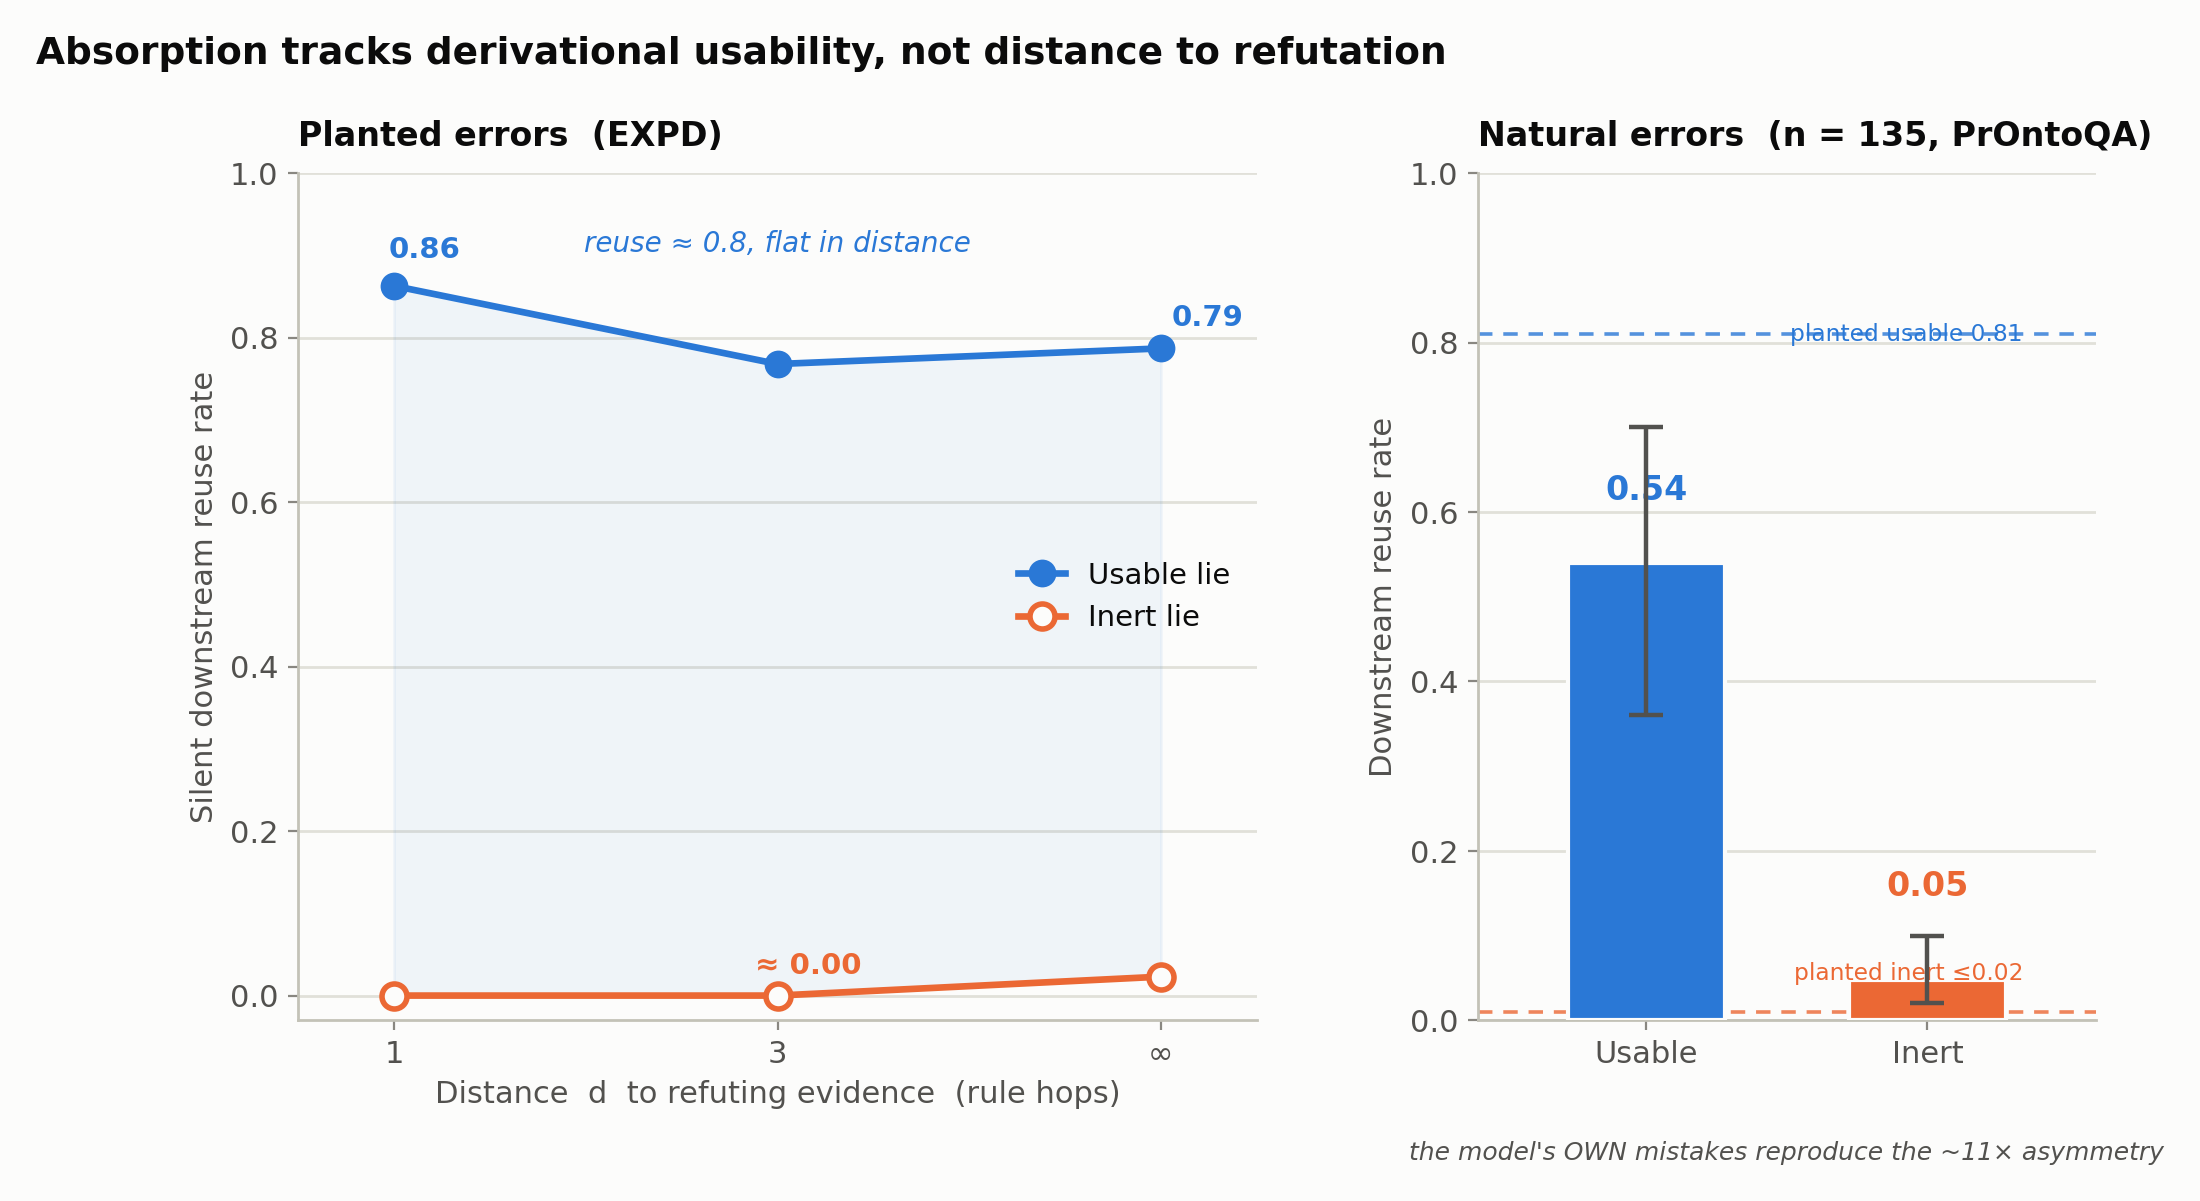
\includegraphics[width=0.86\textwidth]{figures/fig_c_usability_asymmetry.png}
\caption{\textbf{Usability, not distance, governs silent reuse on
Qwen2.5-7B.} Left: silent downstream reuse of a \emph{usable} planted
falsehood is about 0.8 and does not decay as the refuting evidence moves
closer (0.86 / 0.77 / 0.79 at $d{=}1/3/\infty$); \emph{inert} plants sit
near zero. Right: the same asymmetry appears in the model's own natural
errors (usable 0.54, inert 0.05), reproducing the planted direction. The
usable trend is a suggestive observation, not a confirmed effect (the
gradient prediction runs the other way). Natural cell is small and unmatched, so this is
a qualitative match. \emph{Qwen2.5-7B only}; \todo{overlay the per-model
replication showing the usability gap passes on Llama-3.1-8B / Qwen2.5-1.5B
but collapses to 0.013 at 32B (Table~\ref{tab:replication}).}}
% source: figures/FIGURE_CAPTION_PLANS Fig C
\label{fig:usability}
\end{figure}
